\begin{figure}[H]
\centering
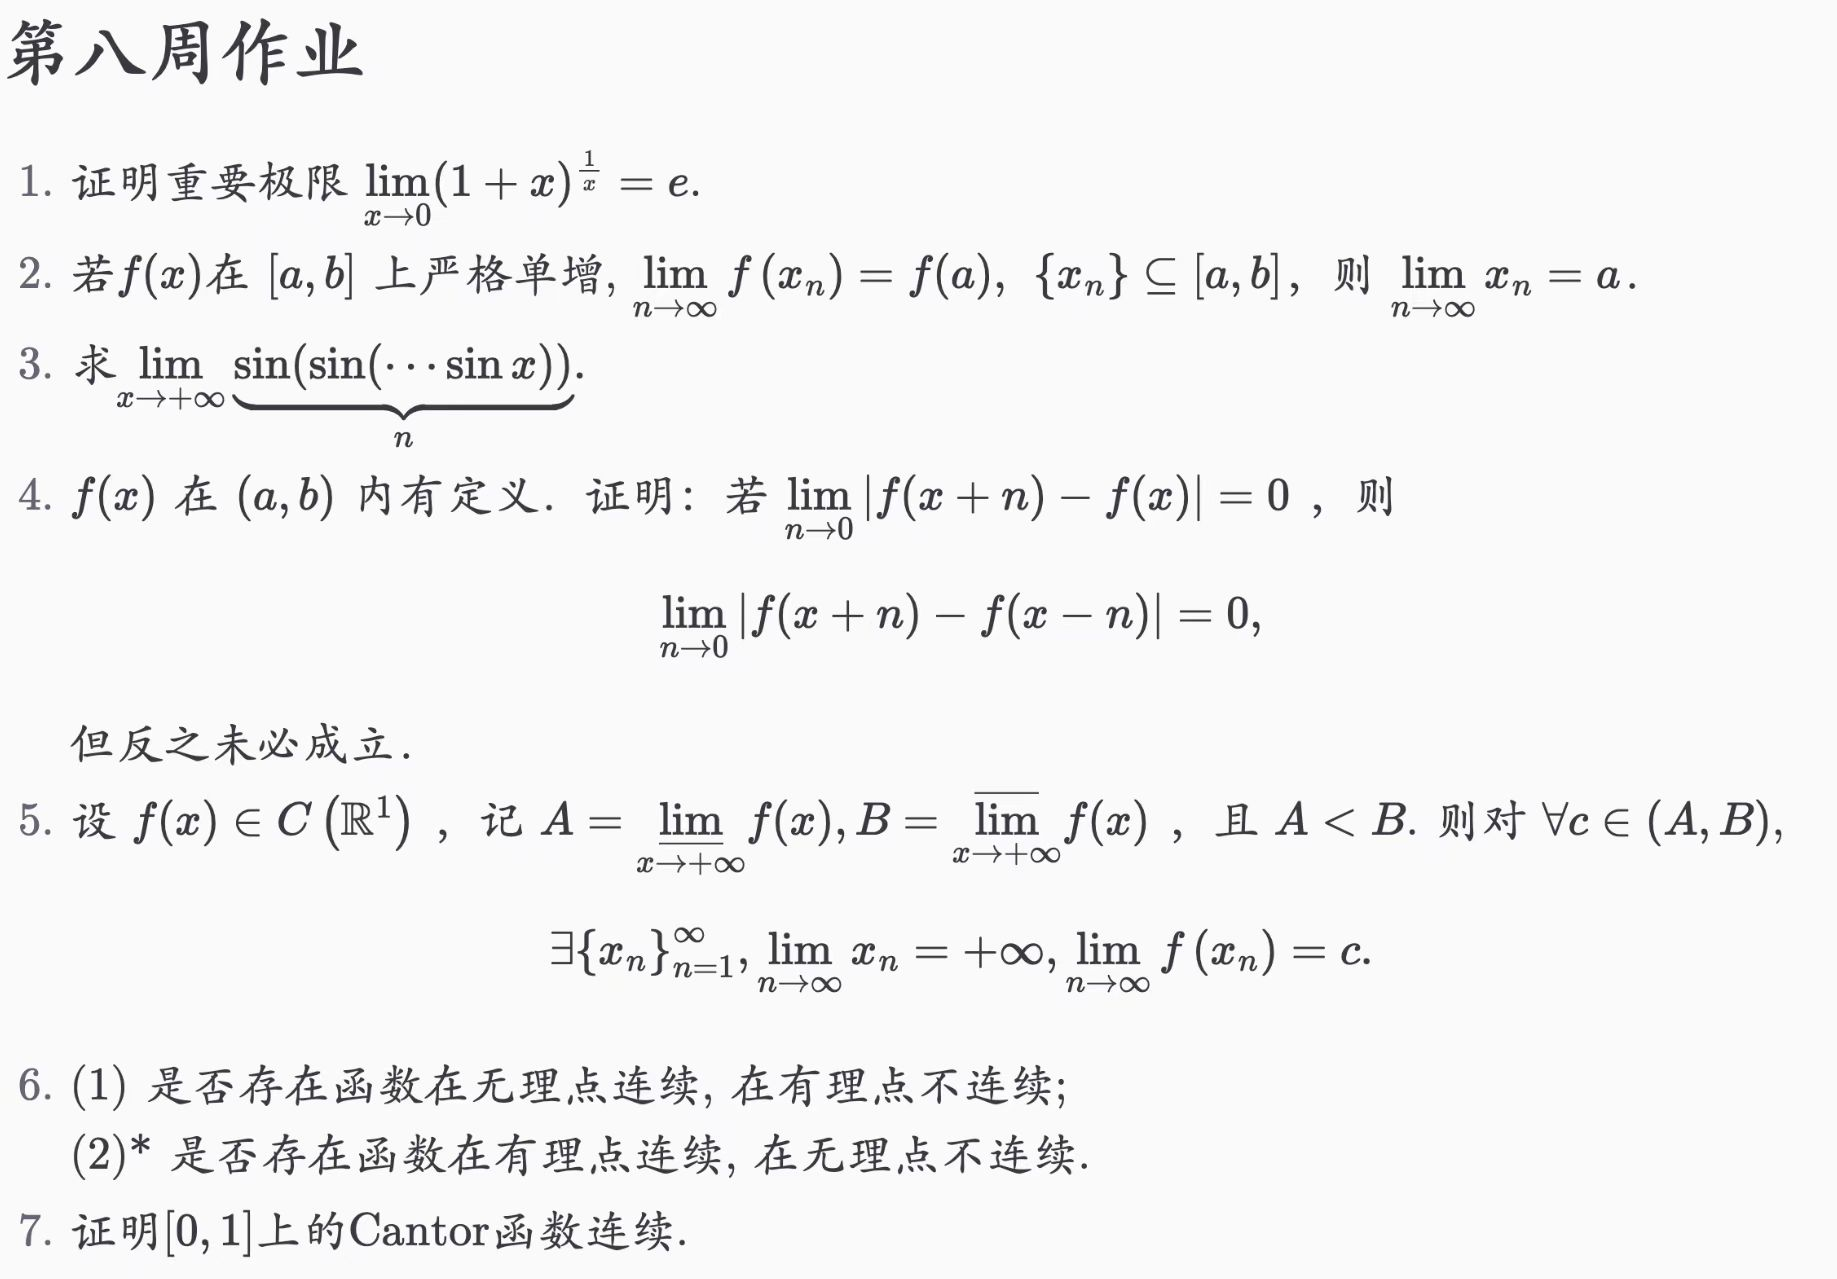
\includegraphics[width=\textwidth]{fc79a56f39495e5f630fe3b481bca532.jpg}
% \caption{}
\label{}
\end{figure}

\begin{exercise}
\begin{enumerate}
		\item Prove the important limit $\lim_{x \rightarrow 0}(1+x)^{\frac{1}{x}}=e$.
	\end{enumerate}
\end{exercise}
\begin{proof}
\[
(1+x)^{\frac{1}{x}}=\exp \left\{  \frac{1}{x}\ln(1+x)  \right\}
\]
\[
\ln (1+x)\coloneqq x-\frac{x^2}{2}+\frac{x^{3}}{3}-\frac{x^{4}}{4}+\dots=\sum_{n=1}^{\infty} \frac{(-1)^{n}x^{n}}{n}
\]
When $\lvert x \rvert<\frac{1}{2}$,
\[
\lvert \ln(1+x)-x \rvert =\left\lvert  \sum_{n=2}^{\infty} \frac{(-1)^{n}x^{n}}{n}  \right\rvert \leq \sum_{n=2}^{\infty} \frac{x^2}{n\cdot2^{n-2}}\leq x^2\cdot \sum_{n=2}^{\infty} \frac{1}{2^{n-1}}=x^2
\]
Thus for $\lvert x \rvert<\frac{1}{2}$,
\[
\left\lvert  \frac{1}{x}\ln(1+x)-1  \right\rvert =\frac{\lvert \ln(1+x)-x \rvert }{\lvert x \rvert }\leq \frac{x^2}{\lvert x \rvert }=\lvert x \rvert
\]
Let $x\to0$, then
\[
\left\lvert  \frac{1}{x}\ln(1+x)-1  \right\rvert \to0
\]
i.e.
\[
\frac{1}{x}\ln(1+x)\to1
\]
Since $f(x)=e^{ x }$ is continuous,
\[
(1+x)^{\frac{1}{x}}=\exp \left\{  \frac{1}{x}\ln(1+x)  \right\}\to e
\]
\end{proof}

\begin{exercise}
2. If $f(x)$ is strictly monotonically increasing on $[a, b]$, $\lim_{n \rightarrow \infty} f(x_n)=f(a),\{x_n\} \subseteq[a, b]$, then $\lim_{n \rightarrow \infty} x_n=a$.
\end{exercise}
\begin{proof}
Since $\lim_{ n \to \infty }f(x_n)=f(a)$ and $f(x)$ is strictly monotonically increasing on $[a,b]$, for any $d\in(a,b]$, there exists $N>0$, s.t.
\[
f(a)\leq f(x_n)\leq f(d)\qquad \forall n>N
\]
Otherwise $\lim_{ n \to \infty }f(x_n)\geq f(d)>f(a)$ for some $d\in(a,b]$, which is a contradiction. Since $f$ is strictly monotonically increasing, we have
\[
a\leq x_n\leq d\qquad \forall n>N
\]
Thus $\lvert x_n-a \rvert\leq d-a$. Since $d$ is arbitrary, we have
\[
\lim_{ n \to \infty } x_n=a
\]
\end{proof}

\begin{exercise}
3. Find $\lim_{x \rightarrow+\infty} \underbrace{\sin (\sin (\cdots \sin x))}_n$.
\end{exercise}
似乎题出错了.
\begin{figure}[H]
\centering
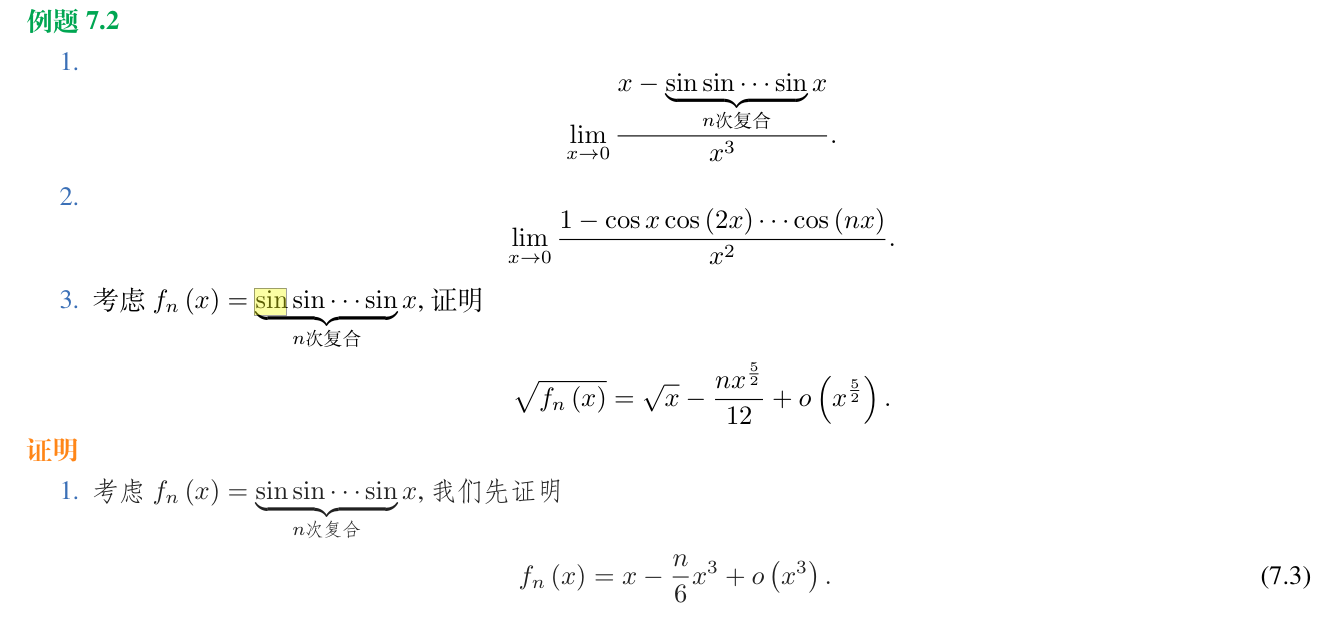
\includegraphics[width=\textwidth]{h-2025041721.png}
% \caption{}
\label{}
\end{figure}
\begin{figure}[H]
\centering
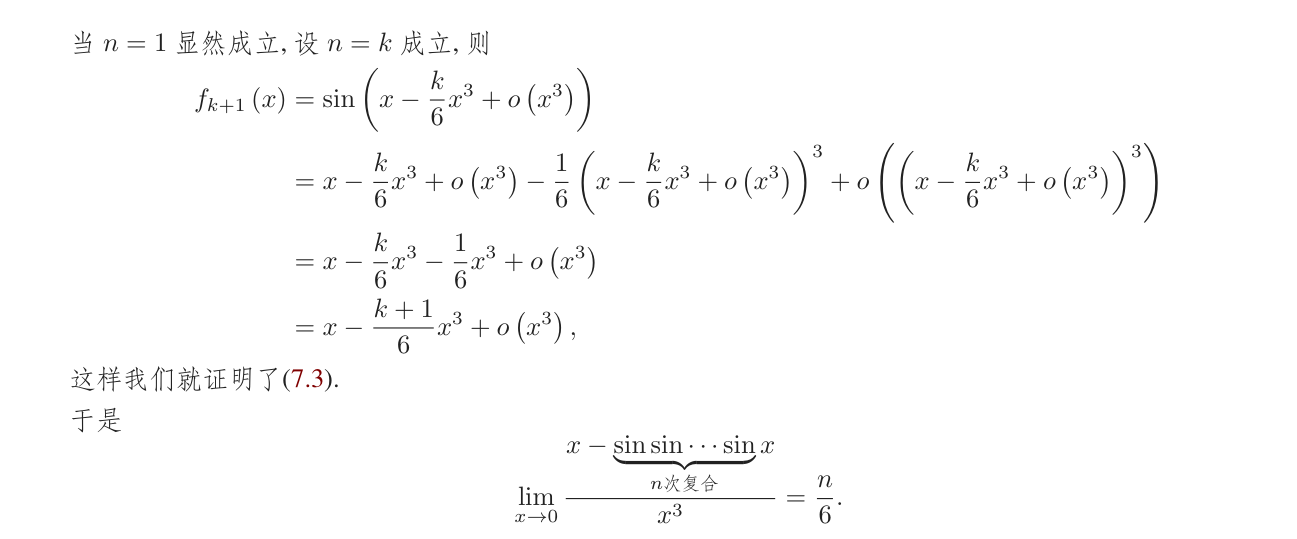
\includegraphics[width=\textwidth]{1-h-2025041721.png}
% \caption{}
\label{}
\end{figure}

\begin{exercise}
4. $f(x)$ is defined in $(a, b)$. Prove that if $\lim_{n \rightarrow 0}|f(x+n)-f(x)|=0$, then
\[
\lim_{n \rightarrow 0}|f(x+n)-f(x-n)|=0,
\]but the converse is not necessarily true.
\end{exercise}
\begin{proof}
If $\lim_{ n \to 0 }\lvert f(x+n)-f(x) \rvert=0$ then for any $\epsilon>0$, there exsits $\delta>0$, s.t.
\[
\lvert f(x+n)-f(x) \rvert <\epsilon \qquad \forall \lvert n \rvert <\delta
\]
Then for any $n\in(-\delta,\delta)$, $-n\in(-\delta,\delta)$, then
\[
\lvert f(x+n)-f(x-n) \rvert \leq \lvert f(x+n)-f(x) \rvert +\lvert f(x-n)-f(x) \rvert <2\epsilon
\]
Thus $\lim_{ n \to 0 }\lvert f(x+n)-f(x-n) \rvert=0$.

Conversely, a conterexample is
\[
f(x)=\begin{cases}
0 & x\in\left( a,\frac{a+b}{2} \right)\cup\left( \frac{a+b}{2},b \right) \\
1 & x=\frac{a+b}{2}
\end{cases}
\]
For $x=\frac{a+b}{2}$, the limit $\lim_{ n \to 0 }\lvert f(x+n)-f(x-n) \rvert=0$ but $\lim_{ n \to 0 }\lvert f(x+n)-f(x) \rvert=1$.
\end{proof}

\begin{exercise}
5. Let $f(x) \in C\left(\mathbb{R}^1\right)$, denote $A=\varliminf_{x \rightarrow+\infty} f(x), B=\varlimsup_{x \rightarrow+\infty} f(x)$, and $A<B$. Then for $\forall c \in(A, B)$,
\[
\exists\left\{x_n\right\}_{n=1}^{\infty}, \lim _{n \rightarrow \infty} x_n=+\infty, \lim _{n \rightarrow \infty} f\left(x_n\right)=c .
\]
\end{exercise}
\begin{proof}
By the definition of $\varlimsup_{ x \to +\infty }$ and $\varliminf_{ x \to +\infty }$, there are two sequences $\{ y_n \}\to \infty$, $\{ z_n \}\to \infty$ s.t.
\[
f(y_n)\to A,\quad f(z_n)\to B\qquad \text{as }n\to \infty
\]
For any $c\in(A,B)$, there are infinitely many elements of $\{ y_n \}$ lying in $(A,c)$, and infinitely many elements of $\{ z_n \}$ lying in $(c,B)$. WLOG, assume that $y_n\in (A, c), z_n\in (c, B),\forall n\in \mathbb{N}$ and $y_n<z_n<y_{n+1}<z_{n+1},\forall n\in \mathbb{N}$. By the continuity of $f$, applying the IVT, there exists $x_n\in(y_n,z_n)$ s.t. $f(x_n)=c$. Thus we have a sequence $\{ x_n \}_{n=1}^{\infty}\to \infty$ with $f(x_n)=c$.
\end{proof}

\begin{exercise}
6. (1) Does there exist a function that is continuous at irrational points and discontinuous at rational points?
(2) $\ast$ Does there exist a function that is continuous at rational points and discontinuous at irrational points?
\end{exercise}
(1) Yes.

\begin{example}
Define Thomae's function $f(x)$ as follows:
\[
f(x)= \begin{cases}1 & \text { if } x=0 \\ 0 & \text { if } x \notin \mathbb{Q} \\ \frac{1}{q} & \text { if } x=\frac{p}{q} \text { in lowest terms }\end{cases}
\]Then $f(x)$ is continuous at every irrational point and discontinuous at every rational point.
\end{example}
(2) No, there does not exist a function that is continuous at rational points and discontinuous at irrational points. The set of points at which a function is continuous must be a $G_\delta$ set (a countable intersection of open sets). The set of rational numbers is not a $G_\delta$ set.

\begin{theorem}
The set of points at which a function is continuous must be a $G_\delta$ set.
\end{theorem}
\begin{proof}
Let $f: \mathbb{R} \rightarrow \mathbb{R}$ be a function. Let $C$ be the set of points at which $f$ is continuous. We want to show that $C$ is a $G_\delta$ set.

For each $x \in \mathbb{R}$ and each $n \in \mathbb{N}$, define
\[
O_n(x)=\bigcup_{y \in \mathbb{R}}\left\{(a, b): x \in(a, b), \sup _{a<y<b} f(y)-\inf _{a<y<b} f(y)<\frac{1}{n}\right\} .
\]
$O_n(x)$ is open for each $n$, since it is the union of open intervals.

We claim that $x \in C$ \textbf{if and only if} for all $n$, $x \in O_n$. In other words, we claim that $x \in C$ if and only if for every $n$ there exists an open interval $(a,b)$ such that $x \in (a,b)$ and $\sup_{a<y<b}f(y)-\inf_{a<y<b}f(y) < \frac{1}{n}$.

Then $x \in C$ if and only if for every $\epsilon>0$ there exists $\delta>0$ such that if $|x-y|<\delta$, then $|f(x)-f(y)|<\epsilon / 2$. Therefore, $x \in C$ if and only if for all $n, x \in O_n$.

Thus, $C=\bigcap_{n=1}^{\infty} O_n$. Since each $O_n$ is open, $C$ is a $G_\delta$ set.

Now we prove the \textbf{if and only if} statement.

$(\Rightarrow)$ If $f$ is continuous at $x$, then for every $\epsilon>0$, there exists $\delta>0$ such that if $|x-y|<\delta$, then $|f(x)-f(y)|<\epsilon / 2$. Let $a=x-\delta$ and $b=x+\delta$, then $x \in(a, b)$ and $\sup _{a<y<b} f(y)-\inf _{a<y<b} f(y)<\epsilon$. So $x \in O_n$ for all $n$.

$(\Leftarrow)$ If for all $n$, $x \in O_n$, then for every $n$ there exists an open interval $(a, b)$ such that $x \in(a, b)$ and $\sup _{a<y<b} f(y)-\inf _{a<y<b} f(y)<1 / n$. Let $\epsilon>0$ be given. Choose $n$ large enough such that $1 / n<\epsilon / 2$. Then there exists an open interval $(a, b)$ such that $x \in(a, b)$ and $\sup _{a<y<b} f(y)-\inf _{a<y<b} f(y)<\epsilon / 2$. Choose $\delta>0$ such that $(x-\delta, x+\delta) \subseteq(a, b)$. Then if $|x-y|<\delta$ then $|f(x)-f(y)|<\epsilon / 2$. So $f$ is continuous at $x$.
\end{proof}

\begin{exercise}
7. Prove that the Cantor function on $[0,1]$ is continuous.
\end{exercise}
\begin{definition}[Cantor function]
The \textbf{Cantor function} is defined as follows:
	\begin{enumerate}
		\item Write $x \in[0,1]$ in base 3 : $x=\sum_{i=1}^{\infty} a_i 3^{-i}$ where $a_i \in\{0,1,2\}$.
		\item If $x$ has a 1 in its ternary expansion, truncate the expansion at the first occurrence of a 1. Change every digit after that first 1 to 0.
		\item Replace all 2's with 1's.
		\item Interpret the result as a binary number.
	\end{enumerate}
This gives the value of the Cantor function $F(x)$.
\end{definition}
\begin{proof}
Let $x \in[0,1]$. We want to show that for every $\epsilon > 0$, there exists a $\delta > 0$ such that if $|y - x| < \delta$, then $|F(y) - F(x)| < \epsilon$.

Let $\epsilon > 0$. Choose $n$ such that $2^{-n} < \epsilon$.

Choose $\delta = 3^{-n}$. Suppose $|y - x| < \delta = 3^{-n}$.

Write $x = \sum_{i=1}^\infty a_i 3^{-i}$ and $y = \sum_{i=1}^\infty b_i 3^{-i}$.

Since $|y - x| < 3^{-n}$, we must have $a_i = b_i$ for all $i = 1, \dots, n-1$.

Let $x' = \sum_{i=1}^\infty a_i' 2^{-i}$ and $y' = \sum_{i=1}^\infty b_i' 2^{-i}$ be the binary representations of $F(x)$ and $F(y)$ respectively.

Since $a_i = b_i$ for all $i = 1, \dots, n-1$, the first $n-1$ digits of the ternary expansions of $x$ and $y$ are the same.

When we apply the Cantor function, we truncate the ternary expansion at the first occurrence of 1, and then change all 2's to 1's. Therefore, the first $n-1$ digits of the binary expansions of $F(x)$ and $F(y)$ are either the same, or differ by the truncation and replacement rules.

In any case, $|F(x) - F(y)| \leq \sum_{i=n}^\infty 2^{-i} = 2^{-n+1} = 2 \cdot 2^{-n} < 2 \epsilon$.

We can also say $|F(x) - F(y)| \leq 2^{-n} < \epsilon$.

Thus, $F$ is continuous.
\end{proof}
Alternative proof:
\begin{proof}
Let $x \in [0,1]$.

Let $x = \sum_{i=1}^\infty a_i 3^{-i}$ where $a_i \in \{0,1,2\}$.

The Cantor function $F(x)$ is continuous everywhere except at points where $x$ has a 1 in its ternary expansion.

If $x$ has a 1 in its ternary expansion, truncate the expansion at the first occurrence of a 1. Change every digit after that first 1 to 0.

Replace all 2's with 1's.

Interpret the result as a binary number.

Let $x = 0.a_1 a_2 \dots a_n 1 0 0 \dots$ in base 3.

Then $F(x) = 0.b_1 b_2 \dots b_n$ in base 2, where $b_i = a_i$ if $a_i = 0$ and $b_i = 1$ if $a_i = 2$.

Let $y = 0.a_1 a_2 \dots a_n 0 2 2 2 \dots$ in base 3.

Then $F(y) = 0.b_1 b_2 \dots b_n$ in base 2, where $b_i = a_i$ if $a_i = 0$ and $b_i = 1$ if $a_i = 2$.

Since $x = y$, we have $F(x) = F(y)$.

Therefore, $F$ is continuous at $x$.
\end{proof}
